\documentclass{beamer}
\usepackage[T1]{fontenc}
\usepackage[utf8x]{inputenc} 
\usepackage[esperanto]{babel}
%\usepackage{umbcboxes}

\title{Trelliĝu}
\subtitle{ang. ,,get trelled''}
\author{Tomasz Szymula \\ tomasz.szymula@pej.pl}
\institute[PEJ]{
\includegraphics[scale=0.3]{bildoj/pej}}

\date[JES 2015]{Junulara E-Semajno, 2015 Eger}
\subject{}

\usetheme{CambridgeUS}
\usecolortheme{beaver}

\AtBeginSubsection[]
{
  \begin{frame}
    \frametitle{Plano}
    \tableofcontents[currentsubsection]
  \end{frame}
}

\begin{document}
  \frame{\titlepage}
 
 
\section{Pri kio temas}


%%%>>>>>>>>>>>>>>>>>>>>>>>>>>>>>>>>>>>>>>>>>>>>>>>>>>>>>>>>>>>>>>>>>>>>>>>>>>>>>>>>>>>>>>>>>>>>>>
  \begin{frame}
    \frametitle{Pri la trejnado}

	
	\begin{itemize}

		\item Ĝi celas proponi al via organizo ilon kaj metodon kiel plezure kunlabori.
		
		\item Mi tamen ne ofendiĝos se al vi ne plaĉos la ideo, estu verdirema.
	
		\item Mi koncentriĝos sur praktikaj aspektoj de aplikado al E-organizo -- pri teĥnikaĵoj oni povas legi multon en Interreto.
	
		\item Neniu montrota ekzemplo estas artefarita. Ĉiuj devenas de lastjara funkciado de Pola Esperanto-Junularo.
		
		\item Tiuspeca esperanta trejnado okazas la unuan fojon. Memoru fuŝojn, difektojn kaj helpu plibonigi.
				
		\item Prezentaĵo kunmetita en \LaTeX
				
	\end{itemize}
  \end{frame}
%%%<<<<<<<<<<<<<<<<<<<<<<<<<<<<<<<<<<<<<<<<<<<<<<<<<<<<<<<<<<<<<<<<<<<<<<<<<<<<<<<<<<<<<<<<<<<<<<



\subsection{Kia problemo estas?}

%%%>>>>>>>>>>>>>>>>>>>>>>>>>>>>>>>>>>>>>>>>>>>>>>>>>>>>>>>>>>>>>>>>>>>>>>>>>>>>>>>>>>>>>>>>>>>>>>
  \begin{frame}
    \frametitle{Komenco}
    \framesubtitle{Vi havas 20 novajn mesaĝojn.}
    
  \begin{center}
    	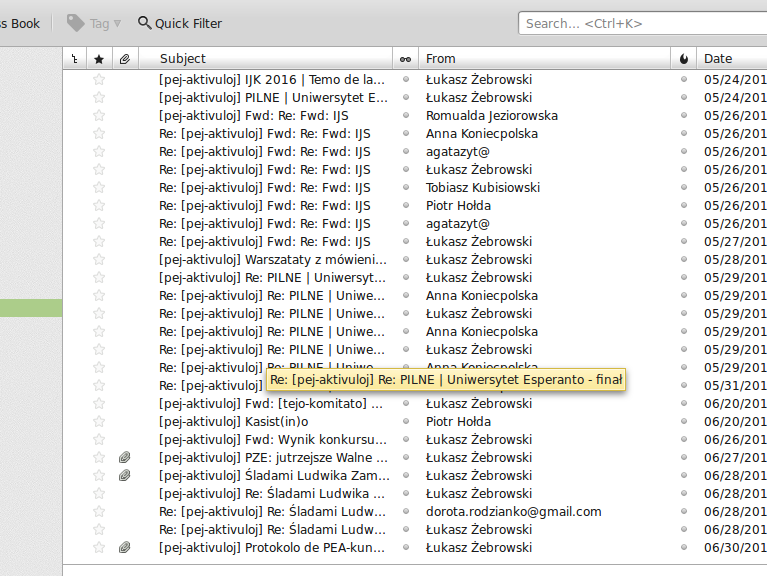
\includegraphics[scale=0.3]{ekranoj/retposhto}
	\end{center}
  \end{frame}
%%%<<<<<<<<<<<<<<<<<<<<<<<<<<<<<<<<<<<<<<<<<<<<<<<<<<<<<<<<<<<<<<<<<<<<<<<<<<<<<<<<<<<<<<<<<<<<<<
 

%%%>>>>>>>>>>>>>>>>>>>>>>>>>>>>>>>>>>>>>>>>>>>>>>>>>>>>>>>>>>>>>>>>>>>>>>>>>>>>>>>>>>>>>>>>>>>>>>
  \begin{frame}
    \frametitle{Retpoŝto}
    \framesubtitle{Ĉu vi ŝatas ĝin uzi por esperantaj projektoj?}
    \begin{itemize}
    	\item Kiom da retadresoj vi uzas?
    	\item Kiom da esperanto-rilataj (nepersonaj = malinteresaj) mesaĝoj vi ricevas semajne?
    	\item Kiom da el ili rilatas rekte al vi?
    	\item Ĉu vi ĉiam (iam ajn?) tuj recivinte la mesaĝon plenumas peton/taskon au prokrastetas?
    \end{itemize}
  \end{frame}
%%%<<<<<<<<<<<<<<<<<<<<<<<<<<<<<<<<<<<<<<<<<<<<<<<<<<<<<<<<<<<<<<<<<<<<<<<<<<<<<<<<<<<<<<<<<<<<<<
   
   
\subsection{Kiel solvi?}
   
%%%>>>>>>>>>>>>>>>>>>>>>>>>>>>>>>>>>>>>>>>>>>>>>>>>>>>>>>>>>>>>>>>>>>>>>>>>>>>>>>>>>>>>>>>>>>>>>>    
  \begin{frame}
    \frametitle{Taskolistoj?}

	\begin{block}{Ekzemplo}
    	\begin{center}
    	
\includegraphics[scale=0.5]{meme/to_do_list}
    	\end{center}
	\end{block}
    
    \begin{itemize}
    	\item Kiel tio helpas?
    	\item Ĉu vi ilin uzas por organizi sian ĉiutagan laboron?
    \end{itemize}
        
  \end{frame}    
%%%<<<<<<<<<<<<<<<<<<<<<<<<<<<<<<<<<<<<<<<<<<<<<<<<<<<<<<<<<<<<<<<<<<<<<<<<<<<<<<<<<<<<<<<<<<<<<<


   
%%%>>>>>>>>>>>>>>>>>>>>>>>>>>>>>>>>>>>>>>>>>>>>>>>>>>>>>>>>>>>>>>>>>>>>>>>>>>>>>>>>>>>>>>>>>>>>>>
  \begin{frame}
    \frametitle{Taskolistoj!}
    %http://www.learningcommons.uoguelph.ca/guides/time_management/html/making_task_list.html
    Ne forgesu, ke:
    \begin{itemize}
    	\item Tio helpas memori eĉ pri flankaj taskoj.
     	\item Oni povas taksi la prioritatojn = sukcesi ĝis limdatoj
        \item Malpli da prokrastado, ĉar vi havos realecan imagon kiom da laboro vere farendas.      
    \end{itemize}
  \end{frame}      
%%%<<<<<<<<<<<<<<<<<<<<<<<<<<<<<<<<<<<<<<<<<<<<<<<<<<<<<<<<<<<<<<<<<<<<<<<<<<<<<<<<<<<<<<<<<<<<<<


\subsection{Trello}
   
%%%>>>>>>>>>>>>>>>>>>>>>>>>>>>>>>>>>>>>>>>>>>>>>>>>>>>>>>>>>>>>>>>>>>>>>>>>>>>>>>>>>>>>>>>>>>>>>>
  \begin{frame}
    \frametitle{Mia propono: Trello.com}
    \begin{center}
    	
\includegraphics[scale=0.4]{bildoj/trello}
    \end{center}    
  \end{frame}
%%%<<<<<<<<<<<<<<<<<<<<<<<<<<<<<<<<<<<<<<<<<<<<<<<<<<<<<<<<<<<<<<<<<<<<<<<<<<<<<<<<<<<<<<<<<<<<<<
  
%%%>>>>>>>>>>>>>>>>>>>>>>>>>>>>>>>>>>>>>>>>>>>>>>>>>>>>>>>>>>>>>>>>>>>>>>>>>>>>>>>>>>>>>>>>>>>>>>
  \begin{frame}
    \frametitle{Kial -- la bildoj sinesprimas.}
    \framesubtitle{Elektu!}
    
	\begin{columns}
    \column{0.5\textwidth}
	    \begin{center}
    		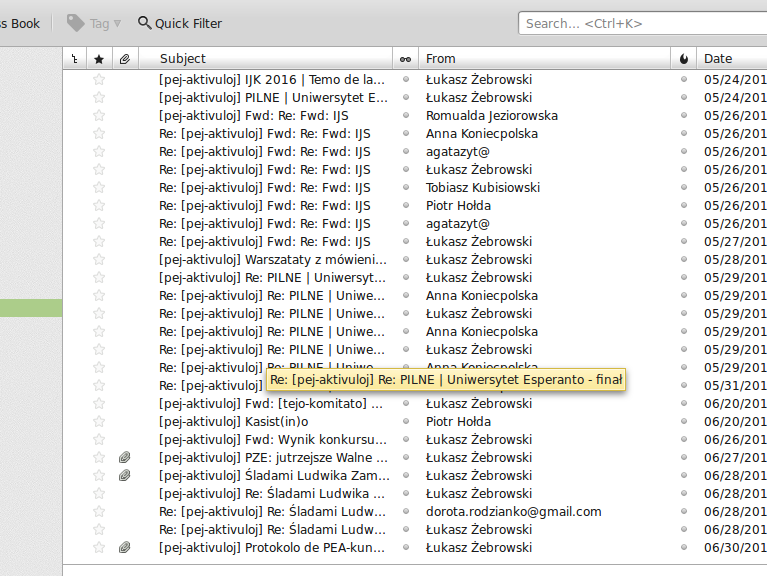
\includegraphics[scale=0.2]{ekranoj/retposhto}
    	\end{center}
	\column{0.5\textwidth}
    	\begin{center}
    	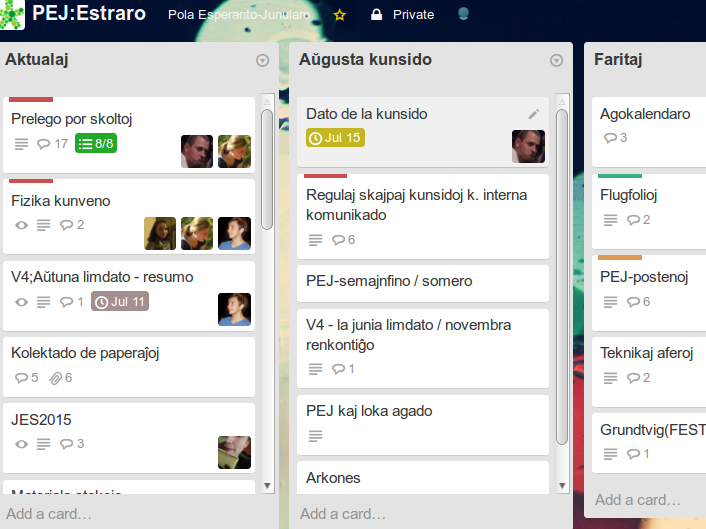
\includegraphics[scale=0.22]{ekranoj/trello-bonas-estraro}
    	\end{center}

	\end{columns}
  \end{frame}
%%%<<<<<<<<<<<<<<<<<<<<<<<<<<<<<<<<<<<<<<<<<<<<<<<<<<<<<<<<<<<<<<<<<<<<<<<<<<<<<<<<<<<<<<<<<<<<<<



%%%>>>>>>>>>>>>>>>>>>>>>>>>>>>>>>>>>>>>>>>>>>>>>>>>>>>>>>>>>>>>>>>>>>>>>>>>>>>>>>>>>>>>>>>>>>>>>>
  \begin{frame}
    \frametitle{Trello - kiu ĝin uzas?}
    
    
  \end{frame}
%%%<<<<<<<<<<<<<<<<<<<<<<<<<<<<<<<<<<<<<<<<<<<<<<<<<<<<<<<<<<<<<<<<<<<<<<<<<<<<<<<<<<<<<<<<<<<<<<
  
  

%%%>>>>>>>>>>>>>>>>>>>>>>>>>>>>>>>>>>>>>>>>>>>>>>>>>>>>>>>>>>>>>>>>>>>>>>>>>>>>>>>>>>>>>>>>>>>>>>
  \begin{frame}
    \frametitle{Ne nur Trello}
    
  \end{frame}
%%%<<<<<<<<<<<<<<<<<<<<<<<<<<<<<<<<<<<<<<<<<<<<<<<<<<<<<<<<<<<<<<<<<<<<<<<<<<<<<<<<<<<<<<<<<<<<<<



%\section{Praktika ekzerco}
\subsection{Uzantkontoj}
%%%>>>>>>>>>>>>>>>>>>>>>>>>>>>>>>>>>>>>>>>>>>>>>>>>>>>>>>>>>>>>>>>>>>>>>>>>>>>>>>>>>>>>>>>>>>>>>>
  \begin{frame}
    \frametitle{Ensalutu en trellon}

	Uzu sian propran Trello konton, Google konton aŭ uzu unu el la subaj:

\begin{center}
	\begin{tabular}{ | c | c | }
	\hline
		uzantnomo & pasvorto \\
	\hline
		blanka.anasero{@}gmail.com & 2anaseroj \\
	\hline
		griza.alaudo{@}gmail.com & 2alaudoj \\
		
%		najtingalo\_trejnanto{@}gmail.com & 2najtingaloj \\
%		kolombo\_trejnanto{@}gmail.com & 2kolomboj\\
	\hline  
	\end{tabular}
\end{center}

\end{frame}
%%%<<<<<<<<<<<<<<<<<<<<<<<<<<<<<<<<<<<<<<<<<<<<<<<<<<<<<<<<<<<<<<<<<<<<<<<<<<<<<<<<<<<<<<<<<<<<<<

%%%>>>>>>>>>>>>>>>>>>>>>>>>>>>>>>>>>>>>>>>>>>>>>>>>>>>>>>>>>>>>>>>>>>>>>>>>>>>>>>>>>>>>>>>>>>>>>>
  \begin{frame}
    \frametitle{Fulmklavoj}
    \framesubtitle{Provu ilin uzi ekzercante!}
    
    \begin{columns}
    \column{0.6\textwidth}
	
	Memoru nur, ke:    
    
	\begin{itemize}
		\item Per klavo ? vi povas rigardi fulmklavaron.
		\item Tre indas tion fari ofte kaj lerni paŝo post paŝo.
	\end{itemize}
    
    	
	\column{0.4\textwidth}
    
    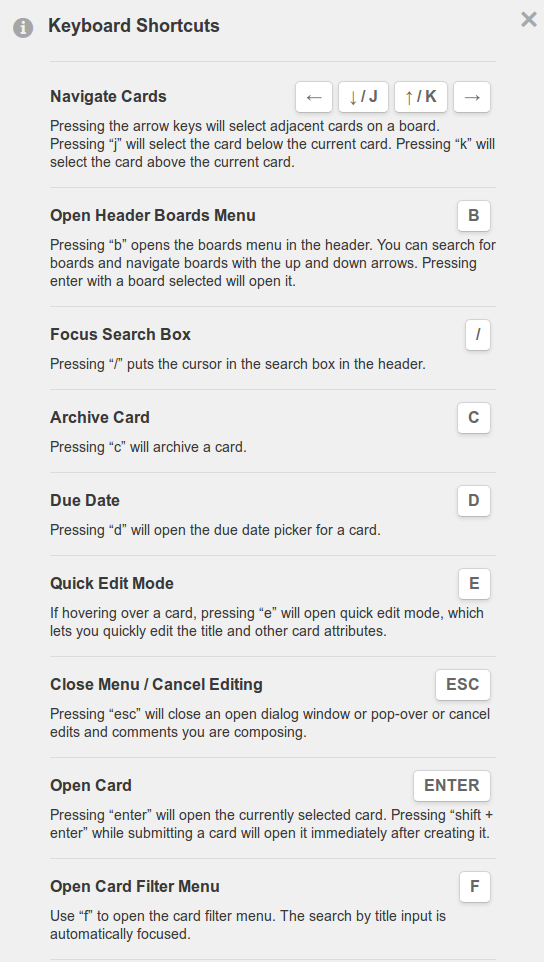
\includegraphics[scale=0.2]{ekranoj/fulmklavaro}
	
	\end{columns}
	
	
  \end{frame}
%%%<<<<<<<<<<<<<<<<<<<<<<<<<<<<<<<<<<<<<<<<<<<<<<<<<<<<<<<<<<<<<<<<<<<<<<<<<<<<<<<<<<<<<<<<<<<<<<




\subsection{Para klakado}
%%%>>>>>>>>>>>>>>>>>>>>>>>>>>>>>>>>>>>>>>>>>>>>>>>>>>>>>>>>>>>>>>>>>>>>>>>>>>>>>>>>>>>>>>>>>>>>>>
  \begin{frame}
    \frametitle{Pariĝu!}
    
    \begin{enumerate}

		\item Decidu kiu unue estos gufujdiĵoranto, kiu gufujkliento.
		\item Ambaŭ personoj havu iun ajn aliron al Trello: telefona aŭ (tabul)komputila. Prefere samtempe, se mankos iloj ni atendos ĝis ĉiuj paroj finos.
		\item Flanka peto: ne malpurigu la komputilojn! :-)
    
    \end{enumerate}
  \end{frame}
%%%<<<<<<<<<<<<<<<<<<<<<<<<<<<<<<<<<<<<<<<<<<<<<<<<<<<<<<<<<<<<<<<<<<<<<<<<<<<<<<<<<<<<<<<<<<<<<<


%%%>>>>>>>>>>>>>>>>>>>>>>>>>>>>>>>>>>>>>>>>>>>>>>>>>>>>>>>>>>>>>>>>>>>>>>>>>>>>>>>>>>>>>>>>>>>>>>
  \begin{frame}
    \frametitle{Ekzerco}
    \framesubtitle{Parto unua}

	\begin{itemize}
		\item Diĵoranto:
		\begin{enumerate}
			\item Kreu tabulon "Posttagmeza menuo".
			\item Agordu tiel, ke la nuraj listoj estu: MENDOJ, SERVITAJ, MENUO.
			\item Aldonu du kartojn: "Vaflo kun dolĉa ŝmiraĵo", "Teo".
			\item Aldonu la klienton al la tabulo.
		\end{enumerate}
			
		\item Kliento:
		\begin{enumerate}
			\item Mendu dolĉaĵon (kreu taŭgan karton en la taŭga listo).
			\item Aldonu la diĵoranton al la karto.
		\end{enumerate}    
	\end{itemize}
	    
  \end{frame}
%%%<<<<<<<<<<<<<<<<<<<<<<<<<<<<<<<<<<<<<<<<<<<<<<<<<<<<<<<<<<<<<<<<<<<<<<<<<<<<<<<<<<<<<<<<<<<<<<

%%%>>>>>>>>>>>>>>>>>>>>>>>>>>>>>>>>>>>>>>>>>>>>>>>>>>>>>>>>>>>>>>>>>>>>>>>>>>>>>>>>>>>>>>>>>>>>>>
  \begin{frame}
    \frametitle{Ekzerco}
    \framesubtitle{Parto dua}

	\begin{itemize}
			
		\item Diĵoranto:
		\begin{enumerate}
			\item Kreu markoliston kun jenaj paŝoj:
				\begin{enumerate}
					\item Difini kia ŝmiraĵo
					\item Servado
					\item Pagado
				\end{enumerate}
				
			\item Demandu kia ŝmiraĵo kaj metu klienton sur la karto.
		\end{enumerate}
				
    
		\item Kliento:
		\begin{enumerate}
			\item Respondu pri ŝmiraĵo, marku ĝustan paŝon sur la markolisto.
			\item Remetu diĵoranton al la karto.
		\end{enumerate}    
		
		\item Diĵoranto:
		\begin{enumerate}
			\item Servu, marku markoliston.
			\item Metu la karton en "SERVITAJ" listo.
		\end{enumerate}    
			
	\end{itemize}		
	
    
  \end{frame}
%%%<<<<<<<<<<<<<<<<<<<<<<<<<<<<<<<<<<<<<<<<<<<<<<<<<<<<<<<<<<<<<<<<<<<<<<<<<<<<<<<<<<<<<<<<<<<<<<


%%%>>>>>>>>>>>>>>>>>>>>>>>>>>>>>>>>>>>>>>>>>>>>>>>>>>>>>>>>>>>>>>>>>>>>>>>>>>>>>>>>>>>>>>>>>>>>>>
  \begin{frame}
    \frametitle{Esenco}
    
	Vi ĉiam strebu \alert{forigi sian vizaĝon de la karto} per:
    
    \begin{itemize}
    	\item plenumo de la peto/tasko,
    	\item klarigo kial ne vi taŭgas (ĉiam trovu anstataŭanton),
    	\item aliaj laŭ via kreemeco, kondiĉe ke kun \alert{fortaj argumentoj} por tio.
    \end{itemize}
    
  \end{frame}
%%%<<<<<<<<<<<<<<<<<<<<<<<<<<<<<<<<<<<<<<<<<<<<<<<<<<<<<<<<<<<<<<<<<<<<<<<<<<<<<<<<<<<<<<<<<<<<<<



\section{Teorio}

\subsection{Sciigoj}

%%%>>>>>>>>>>>>>>>>>>>>>>>>>>>>>>>>>>>>>>>>>>>>>>>>>>>>>>>>>>>>>>>>>>>>>>>>>>>>>>>>>>>>>>>>>>>>>>
  \begin{frame}
    \frametitle{Informado/spamado ekvilibro?}
	\framesubtitle{Ĝenerale...}	
	\begin{block}{I}
		Kiam iu afero rilatas al vi, vi volas esti informata.
	\end{block}
	\begin{block}{II}
		Kiam afero ne rilatas al vi, vi ne volas aŭdi pri ĝi.
	\end{block}
	\begin{block}{III}
		Tamen en libera tempo estus bone havi eblecon trarigardi, kio okazas.
	\end{block}
	
  \end{frame}
%%%<<<<<<<<<<<<<<<<<<<<<<<<<<<<<<<<<<<<<<<<<<<<<<<<<<<<<<<<<<<<<<<<<<<<<<<<<<<<<<<<<<<<<<<<<<<<<<


%%%>>>>>>>>>>>>>>>>>>>>>>>>>>>>>>>>>>>>>>>>>>>>>>>>>>>>>>>>>>>>>>>>>>>>>>>>>>>>>>>>>>>>>>>>>>>>>>
  \begin{frame}
    \frametitle{Kio estas sciigo en Trello?}

	\begin{enumerate}
		\item Sendita retpoŝtmesaĝo (\alert{agordeblas kiom ofte})
		\item Novaĵoj ĉe trello.com
		\item Android/iPhone/Windows Phone sciigo
	\end{enumerate}
	
  \end{frame}
%%%<<<<<<<<<<<<<<<<<<<<<<<<<<<<<<<<<<<<<<<<<<<<<<<<<<<<<<<<<<<<<<<<<<<<<<<<<<<<<<<<<<<<<<<<<<<<<<


%%%>>>>>>>>>>>>>>>>>>>>>>>>>>>>>>>>>>>>>>>>>>>>>>>>>>>>>>>>>>>>>>>>>>>>>>>>>>>>>>>>>>>>>>>>>>>>>>
  \begin{frame}
    \frametitle{Agordoj de sciigoj}
	\begin{columns}
    \column{0.4\textwidth}
	    \begin{block}{Unue eniru agordojn}
	    	\begin{center}
	     	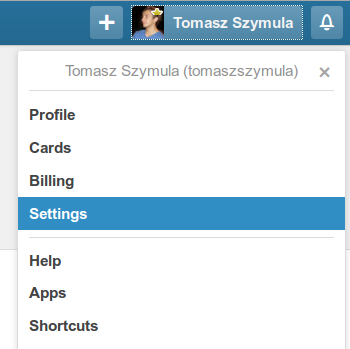
\includegraphics[scale=0.35]{ekranoj/eniru-agordojn}
	    	\end{center}
    	\end{block}
	\column{0.4\textwidth}
    	\begin{block}{Kaj trovu ĝustan sekcion}
    		\begin{center}
    		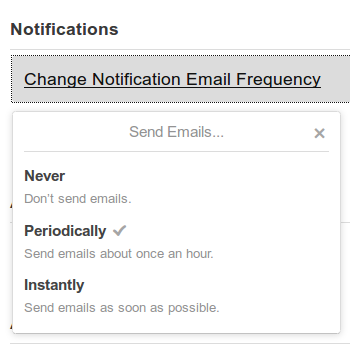
\includegraphics[scale=0.35]{ekranoj/sciigoj-agordo}
    		\end{center}
    	\end{block}

	\end{columns}
  \end{frame}
%%%<<<<<<<<<<<<<<<<<<<<<<<<<<<<<<<<<<<<<<<<<<<<<<<<<<<<<<<<<<<<<<<<<<<<<<<<<<<<<<<<<<<<<<<<<<<<<<


\subsection{Kartoj}
%%%>>>>>>>>>>>>>>>>>>>>>>>>>>>>>>>>>>>>>>>>>>>>>>>>>>>>>>>>>>>>>>>>>>>>>>>>>>>>>>>>>>>>>>>>>>>>>>
  \begin{frame}
    \frametitle{Kion signifas vizaĝo sur karto?}
    \framesubtitle{Amrilato: ,,Tio estas komplika''}

	Eblas diversmaniere kompreni la fakton, ke iu estas ligita al la karto. Rekomendindas (laŭ PEJ spertoj) interkonsenti, ke estas kvar eblecoj:
	\begin{enumerate}
		\item vi \textbf{devas fari ion konkretan},
		\item vi \textbf{devas fari ion konkretan},
		\item vi \textbf{devas fari ion konkretan},
		\pause
		\item aŭ\dots \pause hispana inkvizicio \alert{(neniu atendis!)}.
	\end{enumerate}

  \end{frame}
%%%<<<<<<<<<<<<<<<<<<<<<<<<<<<<<<<<<<<<<<<<<<<<<<<<<<<<<<<<<<<<<<<<<<<<<<<<<<<<<<<<<<<<<<<<<<<<<<


%%%>>>>>>>>>>>>>>>>>>>>>>>>>>>>>>>>>>>>>>>>>>>>>>>>>>>>>>>>>>>>>>>>>>>>>>>>>>>>>>>>>>>>>>>>>>>>>>
  \begin{frame}
    \frametitle{Abonado de kartoj}
    \framesubtitle{Ja aboneblas ĝuste samkiel Kontakto!}
		
	Se vi bezonas nur esti informata, sed ankoraŭ ne havas konkretajn taskojn pri la temo ne aldonu sin al la karto -- \alert{ekzistas aliaj rimedoj por tio}:
	\begin{enumerate}
		\item abonu la karton (ekz. tre grava afero),
		\item abonu la tabulon (ekz. estrareca tabulo)
	\end{enumerate}
	
	\begin{columns}
    \column{0.3\textwidth}
	    \begin{block}{Karto}
	    	\begin{center}
	     	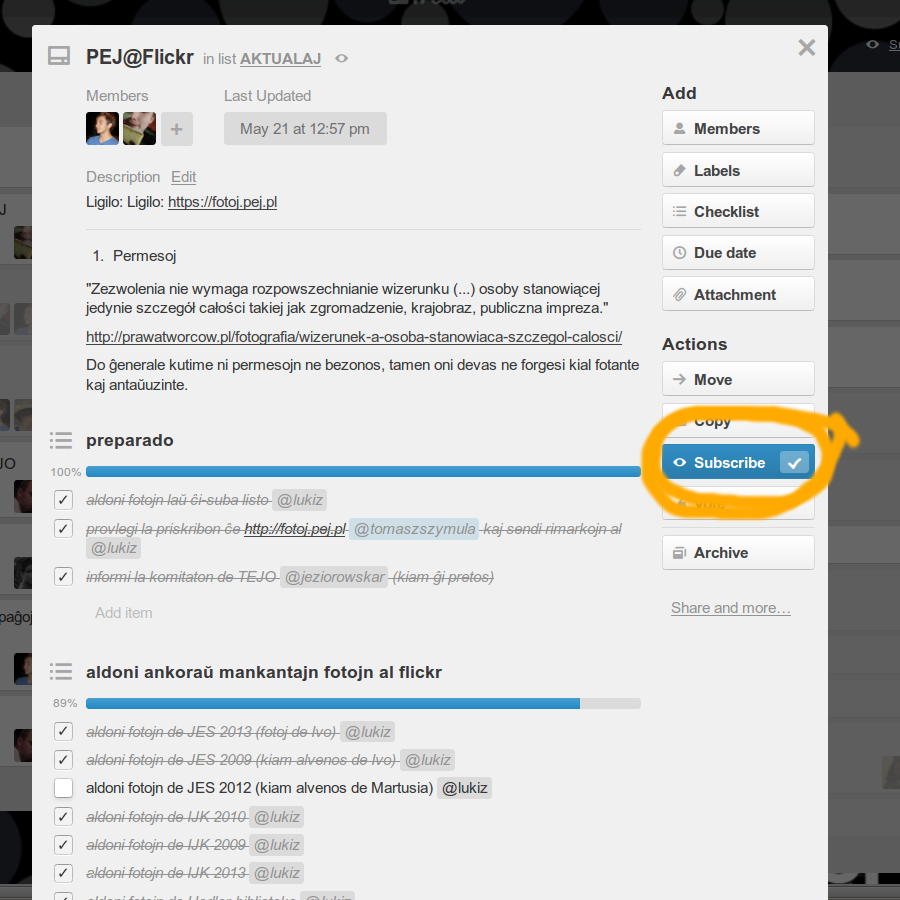
\includegraphics[scale=0.10]{ekranoj/abonu-karton}
	    	\end{center}
    	\end{block}
	\column{0.3\textwidth}
    	\begin{block}{Tabulo}
    		\begin{center}
    		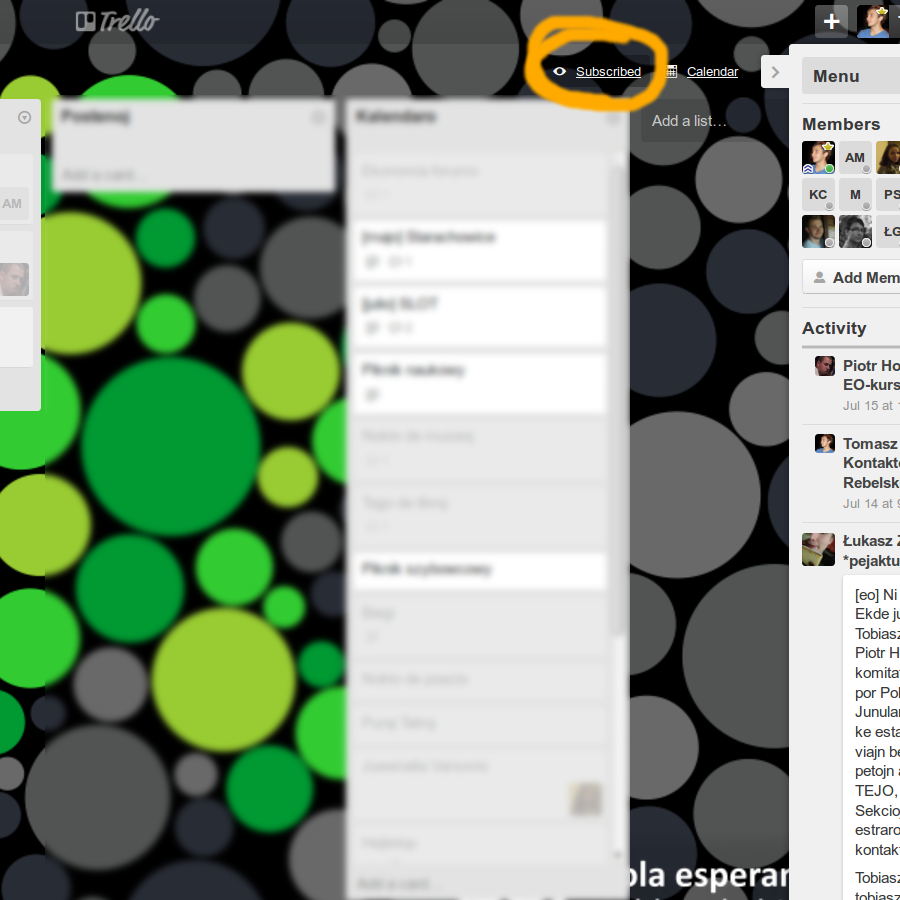
\includegraphics[scale=0.10]{ekranoj/abonu-tabulon}
    		\end{center}
    	\end{block}

	\end{columns}
  \end{frame}
%%%<<<<<<<<<<<<<<<<<<<<<<<<<<<<<<<<<<<<<<<<<<<<<<<<<<<<<<<<<<<<<<<<<<<<<<<<<<<<<<<<<<<<<<<<<<<<<<


%%%>>>>>>>>>>>>>>>>>>>>>>>>>>>>>>>>>>>>>>>>>>>>>>>>>>>>>>>>>>>>>>>>>>>>>>>>>>>>>>>>>>>>>>>>>>>>>>
  \begin{frame}
    \frametitle{Vi kaj la karto}
    \framesubtitle{Ĉu mi menciis tion?}
		
	Same, se vi volas nur informi iun (havigu al tiu persono la sciigon) malrekomendindas meti lin surkarten. Anstataŭ vi povas uzi "Menciu" funkcion.
\begin{center}

	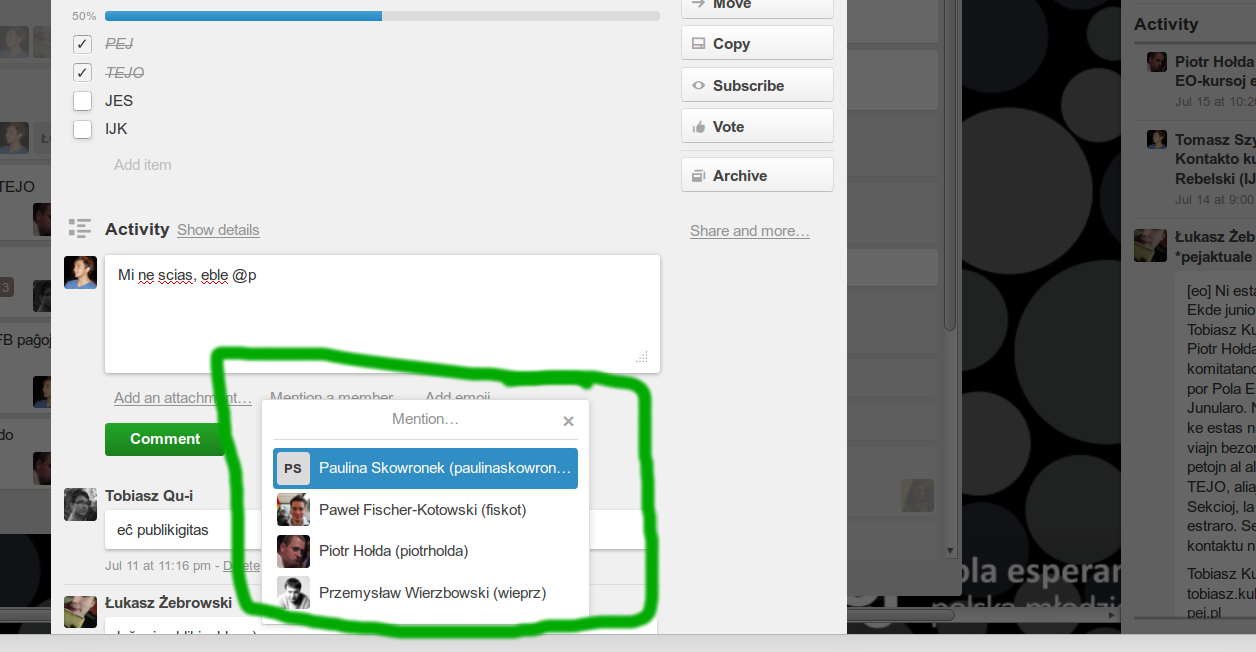
\includegraphics[scale=0.24]{ekranoj/mencio}

\end{center}
  \end{frame}
%%%<<<<<<<<<<<<<<<<<<<<<<<<<<<<<<<<<<<<<<<<<<<<<<<<<<<<<<<<<<<<<<<<<<<<<<<<<<<<<<<<<<<<<<<<<<<<<<

	    

%%%>>>>>>>>>>>>>>>>>>>>>>>>>>>>>>>>>>>>>>>>>>>>>>>>>>>>>>>>>>>>>>>>>>>>>>>>>>>>>>>>>>>>>>>>>>>>>>
  \begin{frame}
    \frametitle{Vi kaj la karto}
    \framesubtitle{Jam vi atendis, ĉu ne?}
	
	\begin{center}
		\begin{block}{Kontrola demando:}
			Kion signifas, se iu metis vin sur iu karto?
		\end{block}
	\end{center}
	
	\begin{center}
	    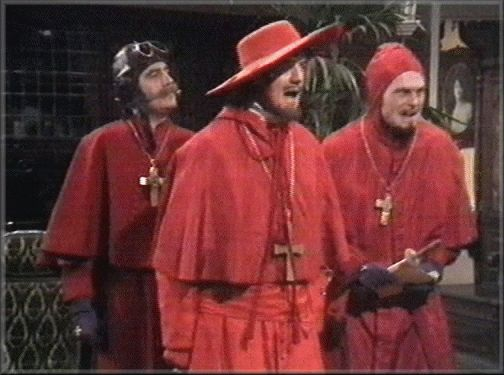
\includegraphics[scale=0.3]{meme/hispana_inkvizicio}
    \end{center}	    
    
  \end{frame}
%%%<<<<<<<<<<<<<<<<<<<<<<<<<<<<<<<<<<<<<<<<<<<<<<<<<<<<<<<<<<<<<<<<<<<<<<<<<<<<<<<<<<<<<<<<<<<<<<
	    

%%%>>>>>>>>>>>>>>>>>>>>>>>>>>>>>>>>>>>>>>>>>>>>>>>>>>>>>>>>>>>>>>>>>>>>>>>>>>>>>>>>>>>>>>>>>>>>>>
%  \begin{frame}
%    \frametitle{Vi kaj la karto}
%    \framesubtitle{Divenu laŭ jenaj informoj:}
%    	
%    \begin{columns}
%    
%    \column{0.45\textwidth}
%    
%    \begin{block}{Kiu reklamos?}
%		
\includegraphics[scale=0.25]{ekranoj/kd-shangho}
%    \end{block}
%    
%    \column{0.45\textwidth}
%        
%    \begin{block}{Kiu verkos?}    
%    	
\includegraphics[scale=0.25]{ekranoj/artikolo-por-tt}
%    \end{block}
%    
%    \end{columns}
%  \end{frame}
%%%%<<<<<<<<<<<<<<<<<<<<<<<<<<<<<<<<<<<<<<<<<<<<<<<<<<<<<<<<<<<<<<<<<<<<<<<<<<<<<<<<<<<<<<<<<<<<<<

%%%>>>>>>>>>>>>>>>>>>>>>>>>>>>>>>>>>>>>>>>>>>>>>>>>>>>>>>>>>>>>>>>>>>>>>>>>>>>>>>>>>>>>>>>>>>>>>>
  \begin{frame}
    \frametitle{Respondeco pri tasko}
    \framesubtitle{Kiel solvi?}

    \begin{columns}
    \column{0.6\textwidth}
    	
    ,,Tradicie'' marku en nomo de la karto. Funkcias sufiĉe bone.
    	
	\column{0.4\textwidth}
    
    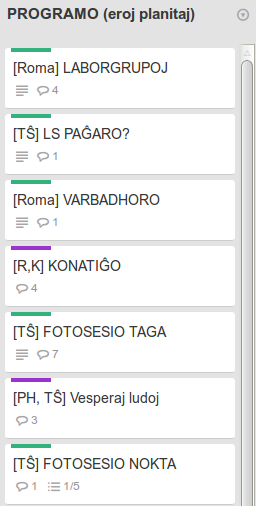
\includegraphics[scale=0.35]{ekranoj/respondeco-pri-karto}
	
	\end{columns}
  \end{frame}
%%%<<<<<<<<<<<<<<<<<<<<<<<<<<<<<<<<<<<<<<<<<<<<<<<<<<<<<<<<<<<<<<<<<<<<<<<<<<<<<<<<<<<<<<<<<<<<<<


%%%%>>>>>>>>>>>>>>>>>>>>>>>>>>>>>>>>>>>>>>>>>>>>>>>>>>>>>>>>>>>>>>>>>>>>>>>>>>>>>>>>>>>>>>>>>>>>>>
%  \begin{frame}
%    \frametitle{Ĉiu projekto bezonas sian kunordiganton}
%
%	\begin{block}{Praktika kaj efika difino}
%		Kunordiganto de la projekto estas tiu, kiu devus honti, se la projekto malsukcesas. Pro tio liŝi zorgu, ke tio ne okazu.
%	\end{block}
%	    
%  \end{frame}
%%%%<<<<<<<<<<<<<<<<<<<<<<<<<<<<<<<<<<<<<<<<<<<<<<<<<<<<<<<<<<<<<<<<<<<<<<<<<<<<<<<<<<<<<<<<<<<<<<


\subsection{Listoj}

%%%>>>>>>>>>>>>>>>>>>>>>>>>>>>>>>>>>>>>>>>>>>>>>>>>>>>>>>>>>>>>>>>>>>>>>>>>>>>>>>>>>>>>>>>>>>>>>>
  \begin{frame}
    \frametitle{Kio sekve?}
    \framesubtitle{Listoj}

	\begin{block}
	
		\begin{center}
		\alert{Laborfluo} difinas kiel oni ŝovas \alert{kartojn} inter \alert{listoj}.
		\end{center}

	\end{block}
		
	%La tabulo estas nur rimedo, kio eĉ pli gravas estas metodaro: tiel nomata  \textbf{laborfluo}. Ĝi difinas kiajn listojn ni havas sur la tablo kaj kiel transmeti la kartojn inter ili.
	
  \end{frame}
%%%<<<<<<<<<<<<<<<<<<<<<<<<<<<<<<<<<<<<<<<<<<<<<<<<<<<<<<<<<<<<<<<<<<<<<<<<<<<<<<<<<<<<<<<<<<<<<<


%%%>>>>>>>>>>>>>>>>>>>>>>>>>>>>>>>>>>>>>>>>>>>>>>>>>>>>>>>>>>>>>>>>>>>>>>>>>>>>>>>>>>>>>>>>>>>>>>
  \begin{frame}
    \frametitle{Listoj: ekzemploj de laborfluoj}
    \framesubtitle{La unua provo}
    
    	\begin{columns}
    \column{0.3\textwidth}
	    \begin{block}
	    
	    	Far\alert{ot}aj
	    	
	    \end{block}
	\column{0.3\textwidth}
    	\begin{block}
    	
    		Far\alert{at}aj
    		
   		\end{block}
	\column{0.3\textwidth}
    	\begin{block}
    	
    		Far\alert{it}aj
    		
    	\end{block}
	\end{columns}
    \vspace{1em}
    	\begin{columns}
    \column{0.5\textwidth}
    Avantaĝoj:
    \begin{itemize}
    		\item simpla
    \end{itemize}
	\column{0.5\textwidth}
    Difektoj:
    \begin{itemize}
    		\item malklara diferenco inter Farotaj kaj Farataj,
    		\item Mankas loko por novaj ideoj, ne nepre tuj farindajn -- ideoj ,,poluas'' nunajn urĝajn taskojn.
    \end{itemize}
    	
	\end{columns}
  \end{frame}
%%%<<<<<<<<<<<<<<<<<<<<<<<<<<<<<<<<<<<<<<<<<<<<<<<<<<<<<<<<<<<<<<<<<<<<<<<<<<<<<<<<<<<<<<<<<<<<<<


%%%>>>>>>>>>>>>>>>>>>>>>>>>>>>>>>>>>>>>>>>>>>>>>>>>>>>>>>>>>>>>>>>>>>>>>>>>>>>>>>>>>>>>>>>>>>>>>>
  \begin{frame}
    \frametitle{Listoj: ekzemploj de laborfluoj}
    \framesubtitle{Dua provo}
    
    	\begin{columns}
    \column{0.3\textwidth}
	    \begin{block}
	    
	    	Ideoj
	    
    	\end{block}
	\column{0.3\textwidth}
    	\begin{block}
    	
    		Aktualaj
    	
    	\end{block}
	\column{0.3\textwidth}
    	\begin{block}
    	
    		Faritaj
    		
    	\end{block}
    	
	\end{columns}
    \vspace{4em}
    	\begin{columns}
    \column{0.5\textwidth}
    Avantaghoj:
    \begin{itemize}
    		\item Ideoj: loko por cerbŝtormetoj
    		\item Aktualaj: la situacio klaras
    \end{itemize}
	\column{0.5\textwidth}
    Difektoj:
    \begin{itemize}
    		\item Aktualaj povas kreski tro longa!
    \end{itemize}
    	
	\end{columns}
  \end{frame}
%%%<<<<<<<<<<<<<<<<<<<<<<<<<<<<<<<<<<<<<<<<<<<<<<<<<<<<<<<<<<<<<<<<<<<<<<<<<<<<<<<<<<<<<<<<<<<<<<


%%%>>>>>>>>>>>>>>>>>>>>>>>>>>>>>>>>>>>>>>>>>>>>>>>>>>>>>>>>>>>>>>>>>>>>>>>>>>>>>>>>>>>>>>>>>>>>>>
  \begin{frame}
    \frametitle{La plej bona solvo?}
    
    		\begin{center}
    		\begin{block}
    		
			\begin{huge}
				\begin{center}
				Estu \alert{fleksebla}!
				\end{center}
			\end{huge} 
    		\end{block}

			\vspace{1.5em}    		
    		
    		
\includegraphics[scale=0.5]{meme/kato}
    		
    		\end{center}

  \end{frame}
%%%<<<<<<<<<<<<<<<<<<<<<<<<<<<<<<<<<<<<<<<<<<<<<<<<<<<<<<<<<<<<<<<<<<<<<<<<<<<<<<<<<<<<<<<<<<<<<<


%%%>>>>>>>>>>>>>>>>>>>>>>>>>>>>>>>>>>>>>>>>>>>>>>>>>>>>>>>>>>>>>>>>>>>>>>>>>>>>>>>>>>>>>>>>>>>>>>
  \begin{frame}
    \frametitle{La plej bona solvo?}
    
    		\begin{center}
    		\begin{block}
    		
			\begin{huge}
				\begin{center}
				\alert{Eksperimentu}!
				\end{center}
			\end{huge} 
    		\end{block}

			\vspace{1em}    		
    		
    		
\includegraphics[scale=0.35]{meme/eksperimento}
    		
    		\end{center}

  \end{frame}
%%%<<<<<<<<<<<<<<<<<<<<<<<<<<<<<<<<<<<<<<<<<<<<<<<<<<<<<<<<<<<<<<<<<<<<<<<<<<<<<<<<<<<<<<<<<<<<<<


%%%>>>>>>>>>>>>>>>>>>>>>>>>>>>>>>>>>>>>>>>>>>>>>>>>>>>>>>>>>>>>>>>>>>>>>>>>>>>>>>>>>>>>>>>>>>>>>>
  \begin{frame}
    \frametitle{Fleksebla?}
    \framesubtitle{Datumoj listo}
    
    
    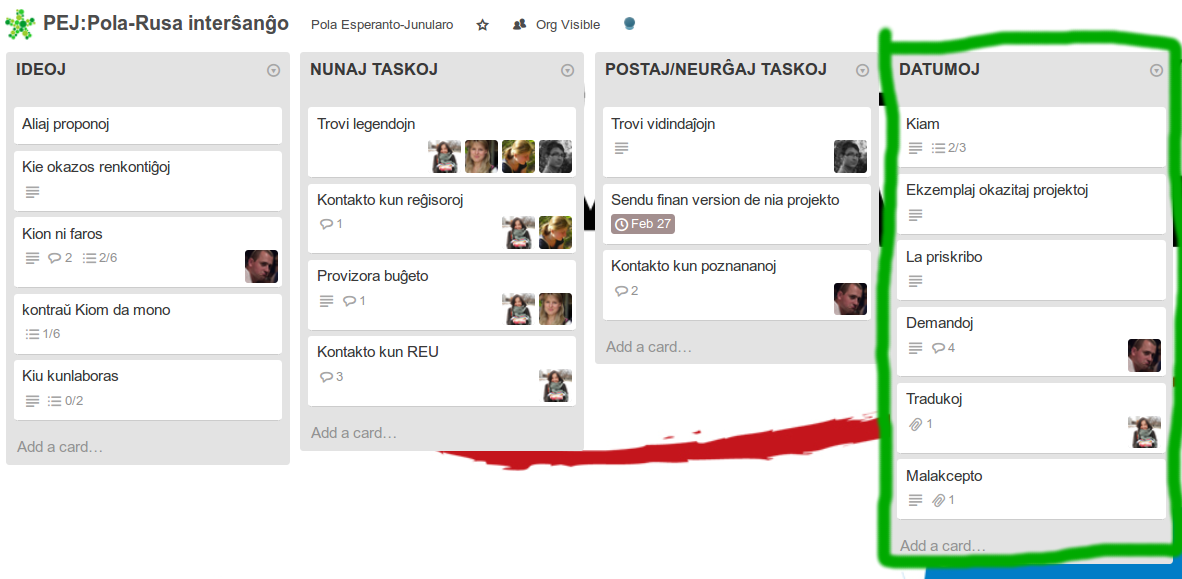
\includegraphics[scale=0.25]{ekranoj/datumoj}

  \end{frame}
%%%<<<<<<<<<<<<<<<<<<<<<<<<<<<<<<<<<<<<<<<<<<<<<<<<<<<<<<<<<<<<<<<<<<<<<<<<<<<<<<<<<<<<<<<<<<<<<<


%%%>>>>>>>>>>>>>>>>>>>>>>>>>>>>>>>>>>>>>>>>>>>>>>>>>>>>>>>>>>>>>>>>>>>>>>>>>>>>>>>>>>>>>>>>>>>>>>
  \begin{frame}
    \frametitle{Fleksebla?}
    \framesubtitle{Listo por priparolindaj aferoj dum skajpa kunsido}
    
    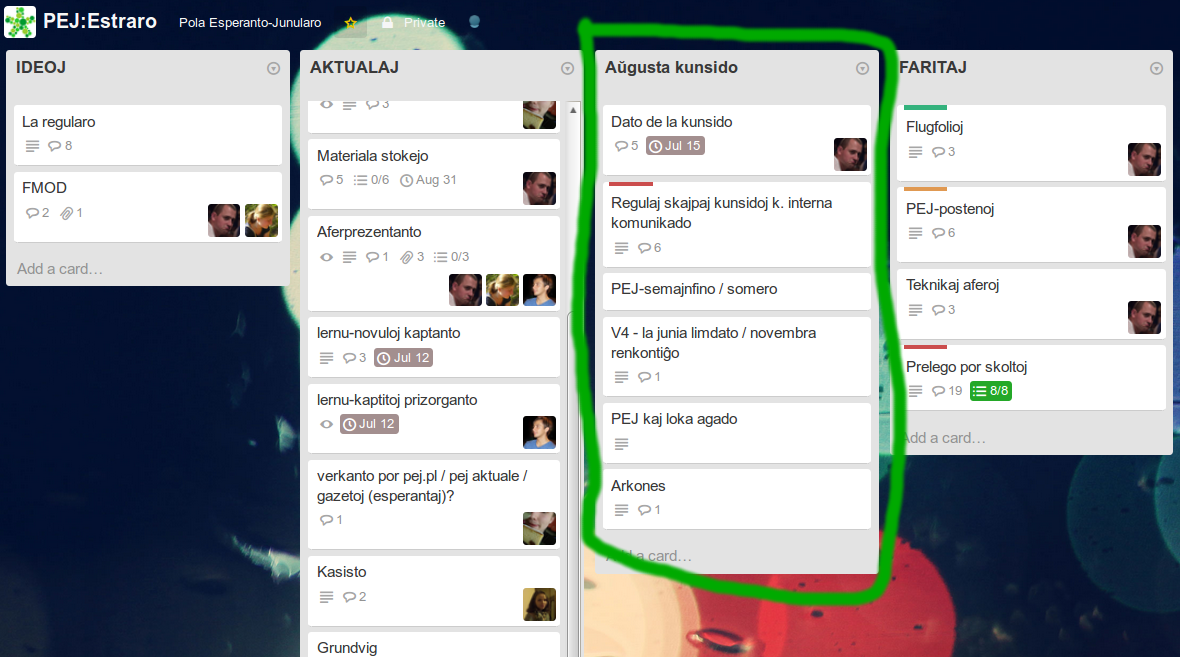
\includegraphics[scale=0.25]{ekranoj/augusta-kunsido}

  \end{frame}
%%%<<<<<<<<<<<<<<<<<<<<<<<<<<<<<<<<<<<<<<<<<<<<<<<<<<<<<<<<<<<<<<<<<<<<<<<<<<<<<<<<<<<<<<<<<<<<<<


%%%>>>>>>>>>>>>>>>>>>>>>>>>>>>>>>>>>>>>>>>>>>>>>>>>>>>>>>>>>>>>>>>>>>>>>>>>>>>>>>>>>>>>>>>>>>>>>>
  \begin{frame}
    \frametitle{Fleksebla?}
    \framesubtitle{Listoj kun programoj por ĉiu tago de aranĝo}
    
    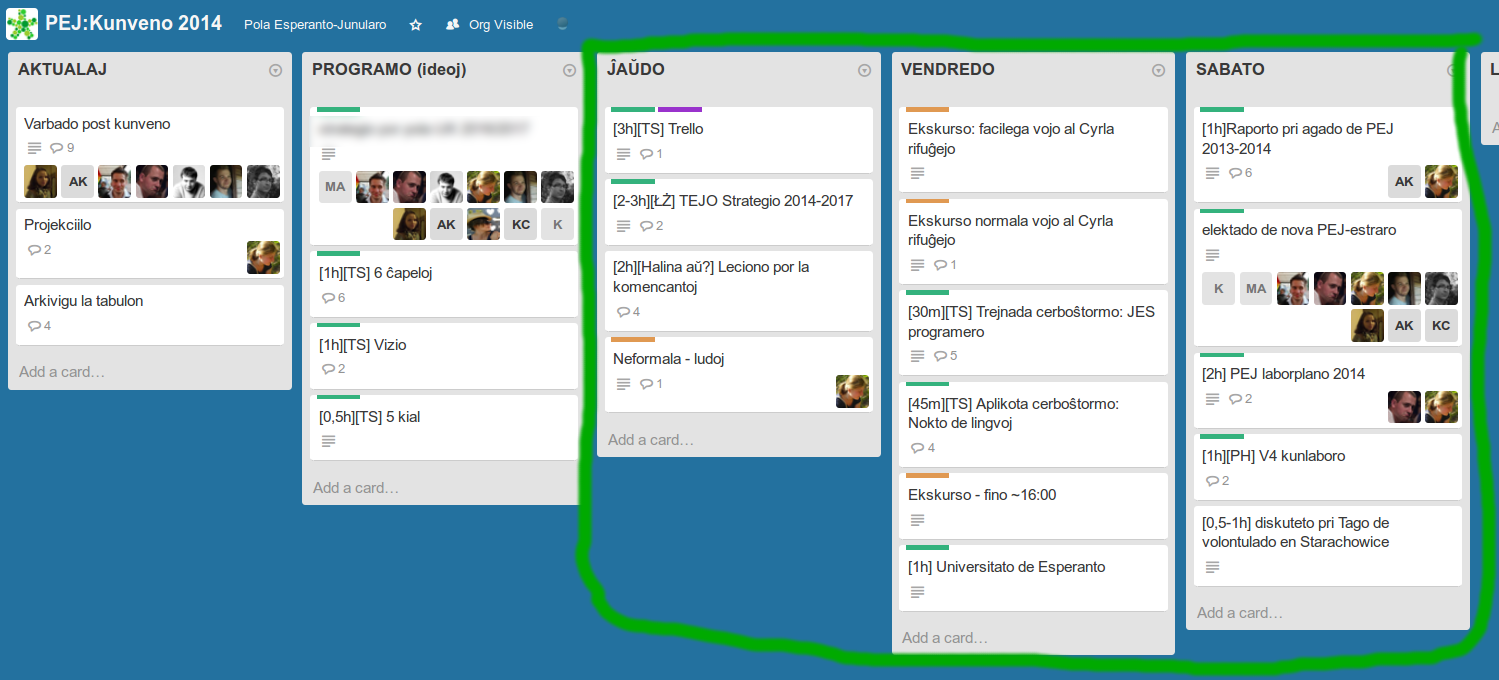
\includegraphics[scale=0.21]{ekranoj/programo-listoj}
  \end{frame}
%%%<<<<<<<<<<<<<<<<<<<<<<<<<<<<<<<<<<<<<<<<<<<<<<<<<<<<<<<<<<<<<<<<<<<<<<<<<<<<<<<<<<<<<<<<<<<<<<

%%%>>>>>>>>>>>>>>>>>>>>>>>>>>>>>>>>>>>>>>>>>>>>>>>>>>>>>>>>>>>>>>>>>>>>>>>>>>>>>>>>>>>>>>>>>>>>>>
  \begin{frame}
    \frametitle{Eksperimentu?}
    \framesubtitle{Ĉi-aŭtune en Krakovo.. publike alirebla tabulo por kursantoj}
    \begin{center}
    
    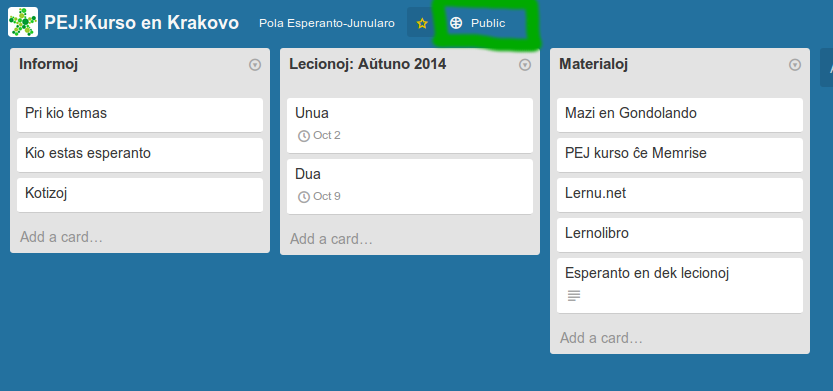
\includegraphics[scale=0.4]{ekranoj/e-kurso}
    \end{center}
  \end{frame}
%%%<<<<<<<<<<<<<<<<<<<<<<<<<<<<<<<<<<<<<<<<<<<<<<<<<<<<<<<<<<<<<<<<<<<<<<<<<<<<<<<<<<<<<<<<<<<<<<


%%%>>>>>>>>>>>>>>>>>>>>>>>>>>>>>>>>>>>>>>>>>>>>>>>>>>>>>>>>>>>>>>>>>>>>>>>>>>>>>>>>>>>>>>>>>>>>>>
  \begin{frame}
    \frametitle{Persona tabulo}
    
    	\begin{columns}
    \column{0.22\textwidth}
	    \begin{block}
	    
	    	Gravaj urĝaj
	    
    	\end{block}
	\column{0.22\textwidth}
    	\begin{block}
    	
    		Negravaj urĝaj
    	
    	\end{block}
	\column{0.22\textwidth}
    	\begin{block}
    	
    		Gravaj neurĝaj
    		
    	\end{block}
	\column{0.22\textwidth}
    	\begin{block}
    	
    		Negravaj neurĝaj
    		
    	\end{block}
    	
	\end{columns}
  \end{frame}
%%%<<<<<<<<<<<<<<<<<<<<<<<<<<<<<<<<<<<<<<<<<<<<<<<<<<<<<<<<<<<<<<<<<<<<<<<<<<<<<<<<<<<<<<<<<<<<<<



 
\subsection{Tabuloj}


%%%>>>>>>>>>>>>>>>>>>>>>>>>>>>>>>>>>>>>>>>>>>>>>>>>>>>>>>>>>>>>>>>>>>>>>>>>>>>>>>>>>>>>>>>>>>>>>>
  \begin{frame}
    \frametitle{Kiom da tabuloj?}

	\begin{columns}
    \column{0.25\textwidth}
	
		Tiom, kiom vi bezonas:
	
	\column{0.75\textwidth}
    
    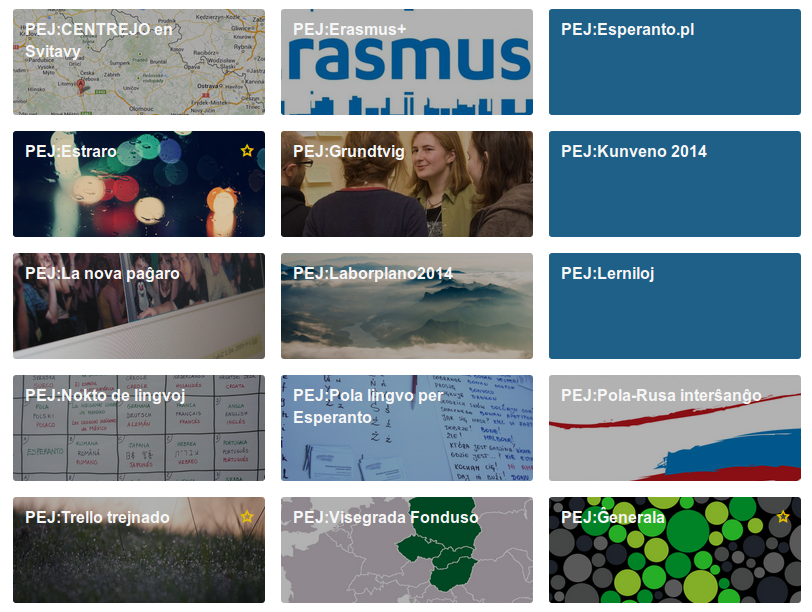
\includegraphics[scale=0.3]{ekranoj/tabuloj}
	
	\end{columns}
	
	
	
  \end{frame}
%%%<<<<<<<<<<<<<<<<<<<<<<<<<<<<<<<<<<<<<<<<<<<<<<<<<<<<<<<<<<<<<<<<<<<<<<<<<<<<<<<<<<<<<<<<<<<<<<


%%%>>>>>>>>>>>>>>>>>>>>>>>>>>>>>>>>>>>>>>>>>>>>>>>>>>>>>>>>>>>>>>>>>>>>>>>>>>>>>>>>>>>>>>>>>>>>>>
  \begin{frame}
    \frametitle{Sendado de kartoj al aliaj tabuloj eblas}
	
	\begin{center}
		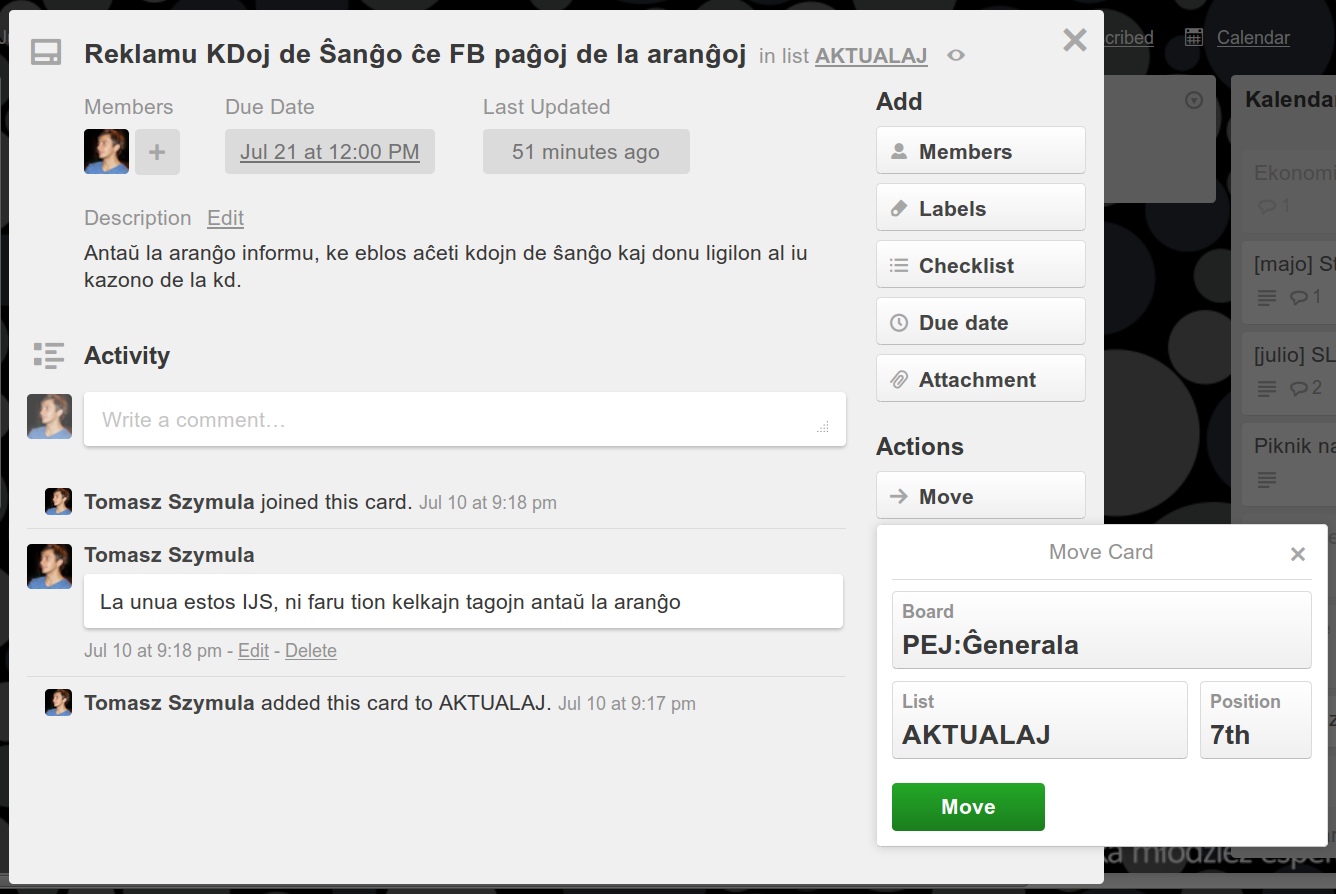
\includegraphics[scale=0.2]{ekranoj/movu-karton}
	\end{center}
	
  \end{frame}
%%%<<<<<<<<<<<<<<<<<<<<<<<<<<<<<<<<<<<<<<<<<<<<<<<<<<<<<<<<<<<<<<<<<<<<<<<<<<<<<<<<<<<<<<<<<<<<<<


%%%>>>>>>>>>>>>>>>>>>>>>>>>>>>>>>>>>>>>>>>>>>>>>>>>>>>>>>>>>>>>>>>>>>>>>>>>>>>>>>>>>>>>>>>>>>>>>>
  \begin{frame}
    \frametitle{Etikedoj}
	\framesubtitle{	,,Ora mezo''}
	
	Ne tro uzu ilin. Mi tamen rekomendas marki almenaŭ la plej gravajn per ruĝa nur por vizuala klareco.
	
  \end{frame}
%%%<<<<<<<<<<<<<<<<<<<<<<<<<<<<<<<<<<<<<<<<<<<<<<<<<<<<<<<<<<<<<<<<<<<<<<<<<<<<<<<<<<<<<<<<<<<<<<




\section{Praktiko}
\subsection{Kartoj 2}

%%%>>>>>>>>>>>>>>>>>>>>>>>>>>>>>>>>>>>>>>>>>>>>>>>>>>>>>>>>>>>>>>>>>>>>>>>>>>>>>>>>>>>>>>>>>>>>>>
  \begin{frame}
    \frametitle{Nomo de kartoj}
		
	Trello havas tre potencan serĉilon. Nomo estu konciza tamen ŝerĉebla ekzemple post du jaroj.
	
	Anstataŭ:
	\begin{itemize}
		\item ,,Paperaĵoj'' -- ,,Pruviloj de la vojaĝo al Italio''.
		\item ,,Renkontiĝo'' -- ,,Renkontiĝo kun la Ĉehoj post Krakovaj Esperantaj Tagoj''.
		\item ,,Afiŝo'' -- ,,JES afiŝo''.
	\end{itemize}
  \end{frame}
%%%<<<<<<<<<<<<<<<<<<<<<<<<<<<<<<<<<<<<<<<<<<<<<<<<<<<<<<<<<<<<<<<<<<<<<<<<<<<<<<<<<<<<<<<<<<<<<<


%%%>>>>>>>>>>>>>>>>>>>>>>>>>>>>>>>>>>>>>>>>>>>>>>>>>>>>>>>>>>>>>>>>>>>>>>>>>>>>>>>>>>>>>>>>>>>>>>
  \begin{frame}
    \frametitle{Priskriboj de kartoj}
			
  	\setbeamercovered{transparent}
  	
	\begin{itemize}
		\item Serĉebleco
		\pause
		\item Kial faru
		\pause
		\item Kion faru
		\pause
		\item Kiu faru
	\end{itemize}
	
  \end{frame}
%%%<<<<<<<<<<<<<<<<<<<<<<<<<<<<<<<<<<<<<<<<<<<<<<<<<<<<<<<<<<<<<<<<<<<<<<<<<<<<<<<<<<<<<<<<<<<<<<

%%%>>>>>>>>>>>>>>>>>>>>>>>>>>>>>>>>>>>>>>>>>>>>>>>>>>>>>>>>>>>>>>>>>>>>>>>>>>>>>>>>>>>>>>>>>>>>>>
  \begin{frame}
    \frametitle{Komentoj sub kartoj}
	
  	\setbeamercovered{transparent}
  		
	\begin{itemize}
		\item Ne spamu
		\pause
		\item Pensu pri tio, kiu ricevos sciigoj
		\pause
		\item Raportu se io okazas, eĉ se neniu demandas
		\pause
		\item Troa afableco: nura ,,Dankon!'' ?
	\end{itemize}
	
  \end{frame}
%%%<<<<<<<<<<<<<<<<<<<<<<<<<<<<<<<<<<<<<<<<<<<<<<<<<<<<<<<<<<<<<<<<<<<<<<<<<<<<<<<<<<<<<<<<<<<<<<


%%%>>>>>>>>>>>>>>>>>>>>>>>>>>>>>>>>>>>>>>>>>>>>>>>>>>>>>>>>>>>>>>>>>>>>>>>>>>>>>>>>>>>>>>>>>>>>>>
  \begin{frame}
    \frametitle{Markolistoj}
    \frametitle{Kion ekzemple signifas: klare difinita tasko}
		
		\begin{center}
		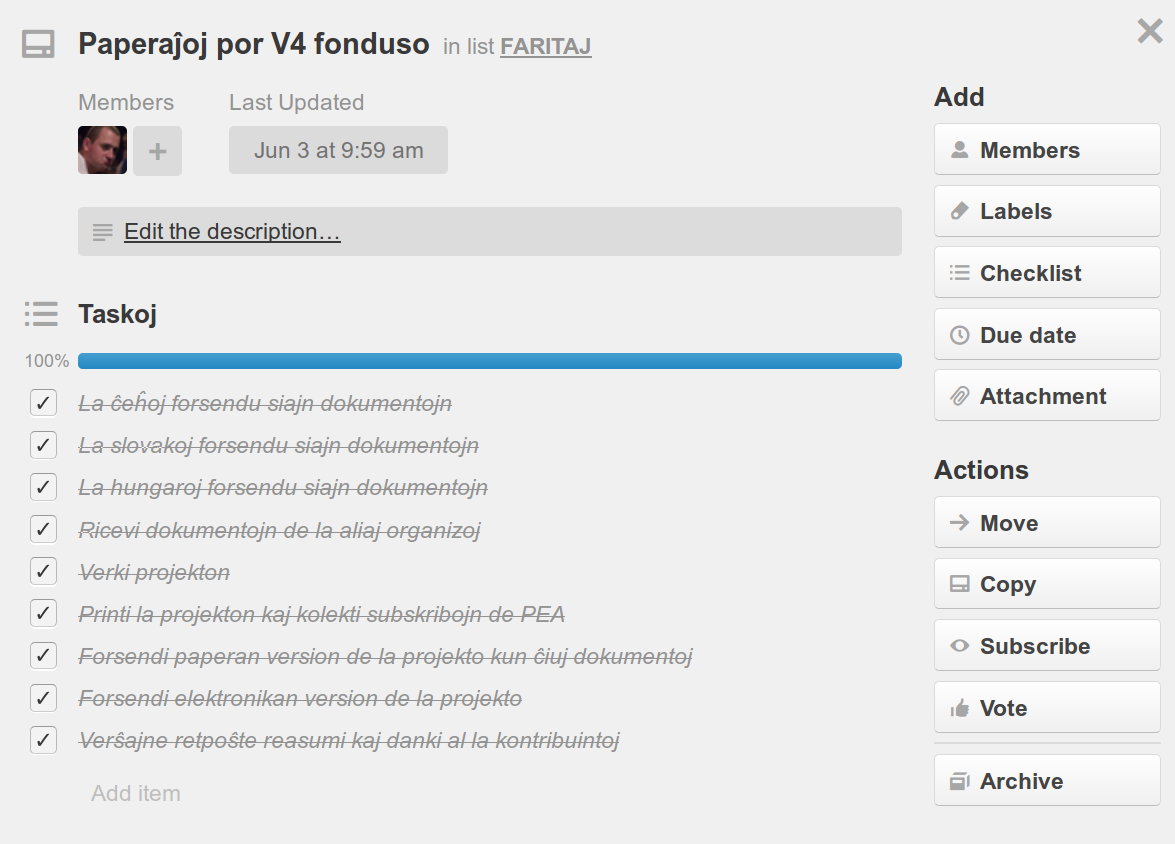
\includegraphics[scale=0.222]{ekranoj/markolistoj}
		\end{center}
	
  \end{frame}
%%%<<<<<<<<<<<<<<<<<<<<<<<<<<<<<<<<<<<<<<<<<<<<<<<<<<<<<<<<<<<<<<<<<<<<<<<<<<<<<<<<<<<<<<<<<<<<<<


%%%>>>>>>>>>>>>>>>>>>>>>>>>>>>>>>>>>>>>>>>>>>>>>>>>>>>>>>>>>>>>>>>>>>>>>>>>>>>>>>>>>>>>>>>>>>>>>>
  \begin{frame}
    \frametitle{Markolistoj + Mencioj}
    \frametitle{Kion ekzemple signifas: klare difinita tasko kun klare difinitaj respondecoj}
    
	\begin{center}
		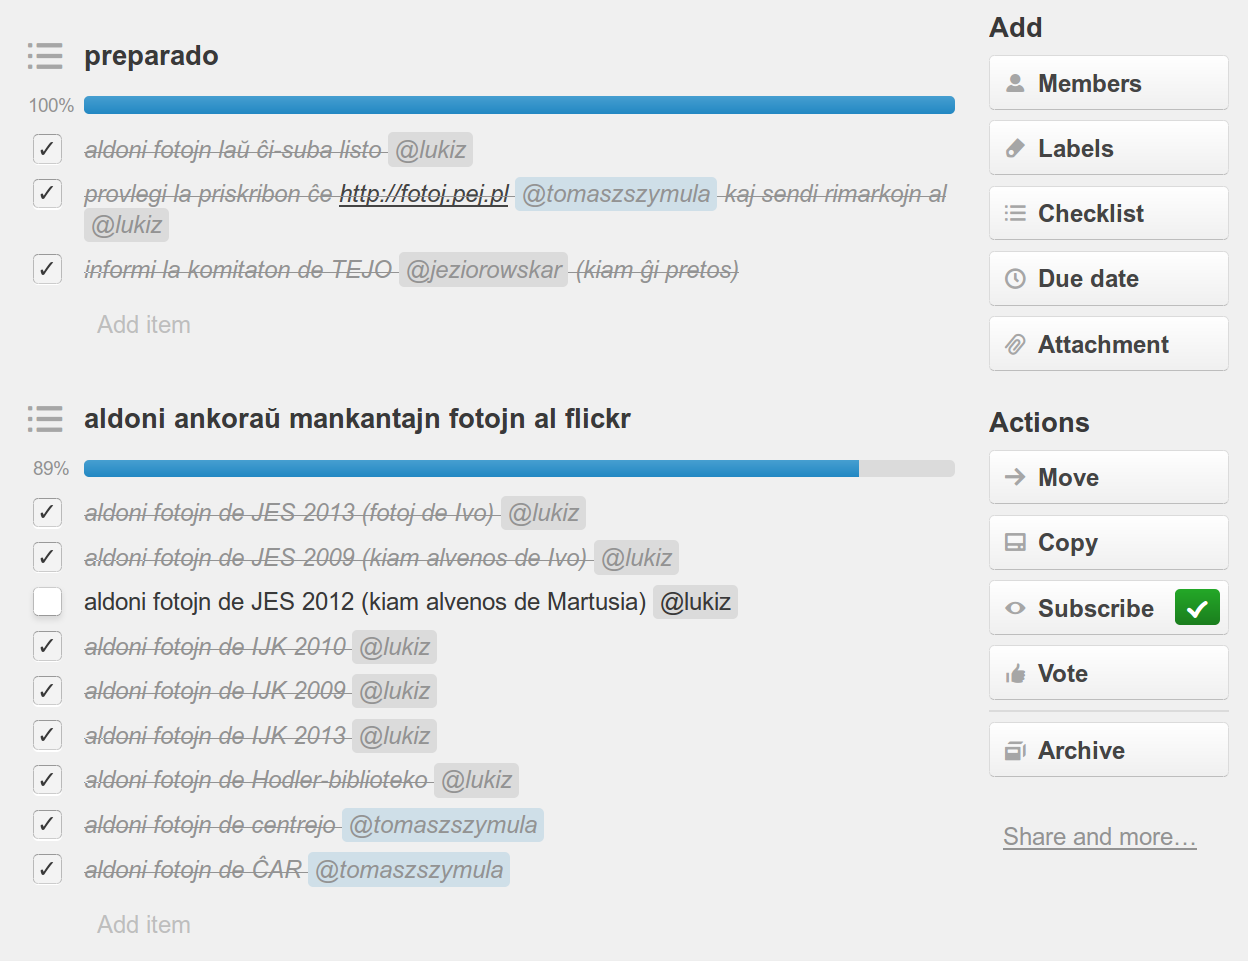
\includegraphics[scale=0.175]{ekranoj/markolistoj-kun-mencioj}
	\end{center}
	
  \end{frame}
%%%<<<<<<<<<<<<<<<<<<<<<<<<<<<<<<<<<<<<<<<<<<<<<<<<<<<<<<<<<<<<<<<<<<<<<<<<<<<<<<<<<<<<<<<<<<<<<<

%%%>>>>>>>>>>>>>>>>>>>>>>>>>>>>>>>>>>>>>>>>>>>>>>>>>>>>>>>>>>>>>>>>>>>>>>>>>>>>>>>>>>>>>>>>>>>>>>
  \begin{frame}
    \frametitle{Limdatoj}
    \frametitle{Kion ekzemple signifas: klare difinite kiam}

    \begin{columns}
    \column{0.6\textwidth}
    
    Tre utilas. Oni ankaŭ ricevas sciigon unu tago antaŭ ĝi.
        	
	\column{0.4\textwidth}
    
    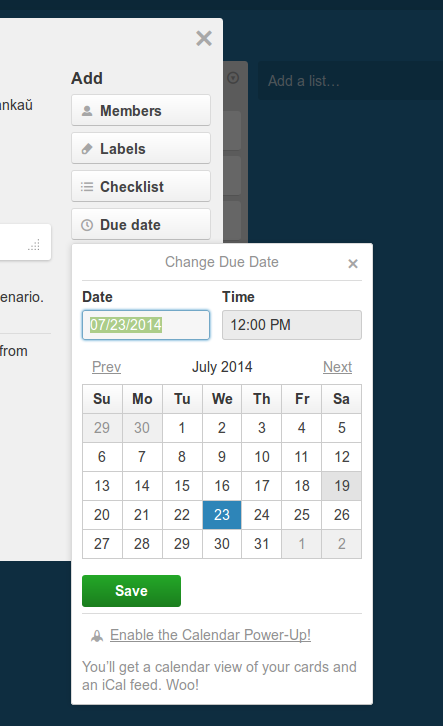
\includegraphics[scale=0.2]{ekranoj/limdato}
	
	\end{columns}
	
	
	
  \end{frame}
%%%<<<<<<<<<<<<<<<<<<<<<<<<<<<<<<<<<<<<<<<<<<<<<<<<<<<<<<<<<<<<<<<<<<<<<<<<<<<<<<<<<<<<<<<<<<<<<<


%%%>>>>>>>>>>>>>>>>>>>>>>>>>>>>>>>>>>>>>>>>>>>>>>>>>>>>>>>>>>>>>>>>>>>>>>>>>>>>>>>>>>>>>>>>>>>>>>
  \begin{frame}
    \frametitle{Etikedoj}
	\framesubtitle{Ne tro uzu}

	\begin{center}
		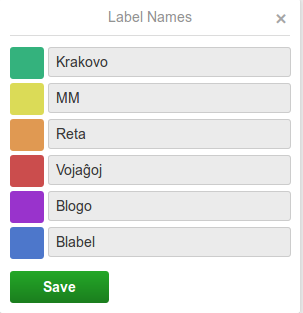
\includegraphics[scale=0.5]{ekranoj/etikedoj}
	\end{center}

  \end{frame}
%%%<<<<<<<<<<<<<<<<<<<<<<<<<<<<<<<<<<<<<<<<<<<<<<<<<<<<<<<<<<<<<<<<<<<<<<<<<<<<<<<<<<<<<<<<<<<<<<



%%%>>>>>>>>>>>>>>>>>>>>>>>>>>>>>>>>>>>>>>>>>>>>>>>>>>>>>>>>>>>>>>>>>>>>>>>>>>>>>>>>>>>>>>>>>>>>>>
  \begin{frame}
    \frametitle{Etikedoj}
	\framesubtitle{Tamen uzu}
	
	
	\begin{center}
		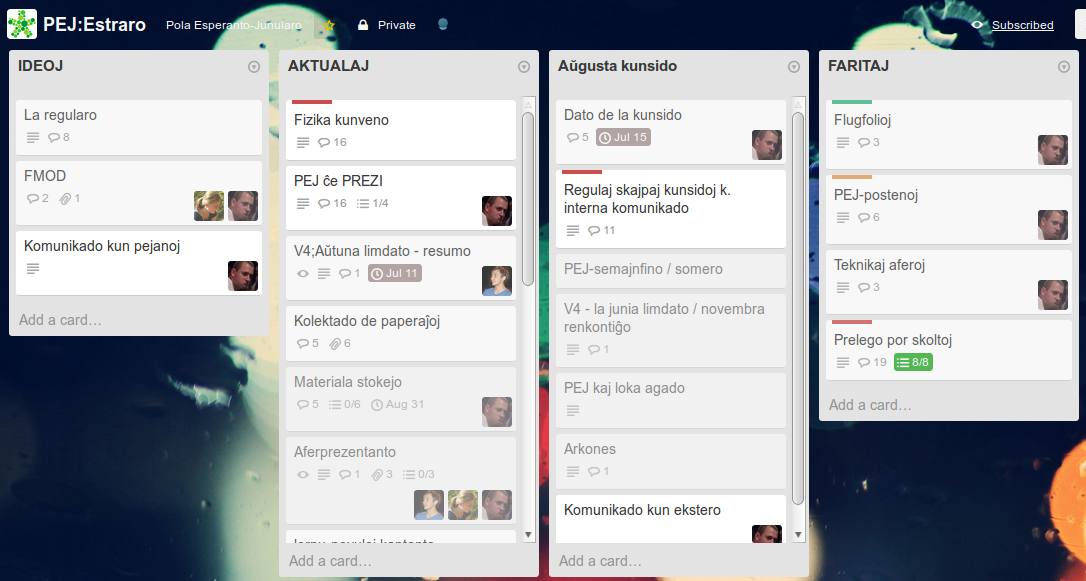
\includegraphics[scale=0.3]{ekranoj/etikedoj-estraro}
	\end{center}

	
  \end{frame}
%%%<<<<<<<<<<<<<<<<<<<<<<<<<<<<<<<<<<<<<<<<<<<<<<<<<<<<<<<<<<<<<<<<<<<<<<<<<<<<<<<<<<<<<<<<<<<<<<



  

\section*{Fino}
%%%>>>>>>>>>>>>>>>>>>>>>>>>>>>>>>>>>>>>>>>>>>>>>>>>>>>>>>>>>>>>>>>>>>>>>>>>>>>>>>>>>>>>>>>>>>>>>>
  \begin{frame}
    \frametitle{Fino}

	\begin{itemize}
		\item Dankon al Vi pro via atento!
		
		\item Antaŭdankon pro viaj rimarkoj (ju pli kritikaj des pli bone)! 
		
	\end{itemize}		
	
  \end{frame}
%%%<<<<<<<<<<<<<<<<<<<<<<<<<<<<<<<<<<<<<<<<<<<<<<<<<<<<<<<<<<<<<<<<<<<<<<<<<<<<<<<<<<<<<<<<<<<<<<


\end{document}
